\chapter{Systemanalyse}\label{chapter:systemanalyse}
Systemanalysen har til formål at finde frem til hvilke procedurer og data der skal bruges til at udforme en løsning af problemet.
Først præsenteres systemdefinitionen, som har udgangspunkt i problemformuleringen de funktionaliteter der blev opstillet i \myref{section:interview2}.
Efterfølgende vil der være henholdsvis analyse af problemområdet og anvendelsesområdet, som sidst i kapitlet vil danne baggrund for en kravspecifikation.

\section{Systemdefinition}
På baggrund af \myref{chapter:problemanalyse} udarbejdes en BATOFF-analyse, som beskrevet i OOA\&D\citep{OOA&D2001}, og efterfølgende formuleres en systemdefinition baseret på disse kriterier.

Denne analyse har til formål at definere retningen for det videre arbejde i projektet.
Systemdefinitionen er en kort tekst, der har til formål at beskrive systemets overordnede krav og funktionaliteter.

Nedenfor ses BATOFF udarbejdelsen og efterfølgende systemdefinitionen.
BATOFF kriterierne hjælper med at danne et overblik over diverse emner, som en systemdefinition bør omfatte.

\subsection{BATOFF}
\begin{description}
\item [Betingelser]\hfill
\begin{itemize}[nolistsep,noitemsep]
\item Adgang til tilbud
\item Interesse for indkøb, opskrifter og tilbud
\end{itemize}

\item [Anvendelsesområde]\hfill
\begin{itemize}[nolistsep,noitemsep]
\item Tilbud
\item Brugere
\item Servere
\item Klienter
\item Overvågning af tilbud
\item Midler til lagring af data
\item Styring af anbefalinger
\end{itemize}

\item [Teknologi]\hfill
\begin{itemize}[nolistsep,noitemsep]
\item Smartphone (Mobil web-device)
\item Tablets
\item Til udvikling: Computer m/udviklerværktøjer
\item Browser m/internetadgang
\end{itemize}

\item [Objekter]\hfill
\begin{itemize}[nolistsep,noitemsep]
\item Opskrifter
\item Indkøbsvarer (tilbud)
\item Brugere
\item Vurdering
\item Præferencer
\item Indkøbsliste
\item Tilbudsaviser
\end{itemize}

\item [Funktioner]\hfill
\begin{itemize}[nolistsep,noitemsep]
\item Overvågning af tilbud
\item Håndtering af indkøbslister
\item Bedømmelse af opskrifter
\end{itemize}

\item [Filosofi]\hfill
\begin{itemize}[nolistsep,noitemsep]
\item Indkøbsassistent og inspirationsgenerering
\end{itemize}
\end{description}



\subsection{Konkret systemdefinition}\label{Sysdef}

Systemet hjælper på problemer, der kan opstå i forbindelse med indkøb og madlavning i hjemmet.
Systemet organiserer indkøbslister, opskrifter og aktuelle tilbudsvarer, samt anbefaler opskrifterne, baseret på bedømmelser af opskrifter og præferencer angående madvarer.
Aktuelle tilbud hentes fra internettet, og kan tilføjes, sammen med generiske varer, til indkøbslister.
Desuden kan det overvåge hvornår, en valgt generisk vare kommer på tilbud.
Systemet tilgås via en webbrowser, således det kan bruges på både computer, tablet og smartphone.
Systemet udvikles som en serverside-applikation med adgang til databaser til håndtering af system- og brugerdata.
Udviklingen af systemet kræver computere med de relevante udviklingsværktøjer.

Denne systemdefinition vil nu være udgangspunkt for vores videre arbejde i rapporten.

\section{Modellering af System}
Ifølge OOA\&D analyseres både problemområdet og anvendelsesområdet for problemet\cite[s. 6]{OOA&D2001}.
Disse er defineret som følgende:

\textit{\textbf{Problemområde:} ''Den del af omgivelserne, der administreres, overvåges eller styres ved hjælp af et system''}

\textit{\textbf{Anvendelsesområde:} ''En organisation, der administrerer, overvåger eller styrer et problemområde''}

\subsection{Problemområdet}
Problemområdet bruges som en modellering af et problem fra den virkelige verden, hvor et system skal benyttes for at administrere, overvåge eller styre et område. 
Dette gøres ved at beskrive diverse klasser, som vil indgå i systemet, ud fra disse ses på hvilke hændelser, som er involveret i klasserne.
Ydermere ses der på, hvilken adfærd der er mellem diverse klasser, hændelser og objekter i systemet.
Dette giver en beskrivelse af, hvilken opførsel og struktur problemområdet skal modellere.
I dette projekt omfatter problemområdet planlægning af indkøb, inspiration til mad samt det at spare penge ved at købe tilbud.
For at beskrive dette nærmere, ses der på klassediagrammer og hændelsestabeller, for at danne overblik over systemet og ende ud med en sammenhængende model for problemområdet.
\subsection{Anvendelsesområdet}
Hvor problemområdet beskriver systemet, beskriver anvendelsesområdet, hvordan systemet skal anvendes.
Ud fra dette spørgsmål opstilles en række af krav for systemets funktioner og grænseflade.
Til dette formål ses der på brugen af systemet, hvilke typer af brugere der er, hvilke brugsmønstre der er for de individuelle funktionaliteter i systemet, samt hvordan funktionaliteterne skal tilgås fra grænsefladen.
I dette projekt indebærer anvendelsesområdet at kunne administrere sine indkøb, få en let oversigt over tilbud, finde inspiration til mad i form af opskrifter, samt at kunne overvåge varer, som man har interesse for at købe på tilbud.


\section{Analyse af problemområde}

Ud fra systemdefinitionen i \myref{Sysdef} ved vi, at systemet skal holde styr på følgende:

\begin{itemize}[noitemsep,nolistsep]
	\item Tilbud
	\item Varer
	\item Indkøbslister
	\item Opskrifter
\end{itemize}

Med disse informationer kan systemet hjælpe brugeren til at finde billige varer i bestemte butikker og eventuelt anbefale opskrifter, der bruger disse tilbudsvarer.
I de følgende afsnit vil disse emner blive beskrevet vha. klassebeskrivelser, en hændelsestabel, og et klassediagram.

\subsection{Klasser}
I dette afsnit vil vi analysere klassernes sammenhæng, derudover vil yderligere klasser blive tilføjet, hvis det findes nødvendigt.

\begin{description}
\item[Vare]\hfill\\
En vare indgår i opskrifter, og indkøbslister.
Når man laver sin indkøbsliste, kan man vælge varer man vil købe, og tilføje dem til indkøbslisten.
Desuden kan en vare have et antal tilbud, hvilket betyder, at der også skal laves en relation til tilbudsklassen.

\item[Tilbud]\hfill\\
Når der kommer nye varer på tilbud, modelleres disse og kobles, vha. en association, til varer.

\item[Opskrift]\hfill\\
En opskrift har en liste over ingredienser, hvilket altså er varer samt mængden af varen.
I interviewene i \myref{section:interview2}, blev det nævnt, at brugerne gerne ville kunne vurdere en opskrift og dermed få anbefalet yderligere opskrifter, som minder om denne.
For at kunne lave vurderinger, skal der laves en vurderingsklasse.

\item[Vurdering]\hfill\\
En vurdering med tal gives for at rangere opskrifter. 
Vurderingen danner også grundlag for, at systemet kan anbefale opskrifter.

\item[Anbefaling]\hfill\\
En anbefaling, af en opskrift, kan gives til personer, når de har givet positive vurderinger af andre opskrifter, som minder om den vurderede opskrift.

\item[Person]\hfill\\
Personklassen gør det muligt at holde styr på forskellige personer, da disse tilsluttes opskrifter, vurderinger, og indkøbsliter.
Derudover vil en person også have præferencer, for butikker de handler i, samt madvarer.

\item[Indkøbsliste]\hfill\\
Indkøbslister laves af en person, og fyldes op med objekter fra vareklassen.
Indkøbslisterne kan deles imellem flere brugere.
\end{description}


\subsection{Hændelser}\label{handelser}
På baggrund af de nævnte funktionaliteter i prototype interviewene, \myref{section:interview2}, er der fundet forskellige hændelser, relevante for funktionaliteterne.
Ud fra disse laves en hændelsestabel, der beskriver, hvilke klasser forskellige hændelser påvirker.
Formålet med, at identificere hændelserne samt at analysere disse i en hændelsestabel, er at forstå problemområdet bedre.
Derved kan det hjælpe med forståelsen for, hvordan en løsning ville kunne designes, for at afhjælpe de problemer, der findes i problemområdet. 
Desuden kan tabellen hjælpe med strukturen på klasserne.
Hvis to klasser har samme hændelser, kan disse klasser ofte tilpasses under én klasse, og dermed opnås en bedre struktur.

\begin{table}[H]
  \centering
    \colorlet{shadecolor}{gray!40}
    \rowcolors{1}{white}{shadecolor}
      \begin{tabular}{l|lccccccc}
      %\hline
       								& \rot{Tilbud}  & \rot{Indkøbsliste} & \rot{Opskrift} & \rot{Vare} & \rot{Person}& \rot{Vurderinger} \\ \hline
      Vare tilføjet til indkøbsliste&               & +      &          & +     & +     &   \\ 
      Vare fjernet fra indkøbsliste	&              	& +      &          & +     & +     &   \\ 
      Vare aftjekket på indkøbsliste&               & +      &          & +     & +     &   \\ 
      Opskrift valgt ???       		& +             & +      &          & +     & +     &   \\ 
      Tilbud oprettet        		& +            	& +      & +        & +     &       &   \\ 
      Tilbud aktiveret        		& +            	& +      & +        & +     &       &   \\ 
      Tilbud udgået          		& +        		& +      & +     	&       &       &   \\ 
      Vare tilføjet til overvågning & +          	&        &          & +     & +     &   \\ 
      Vare fjernet fra overvågning  & +          	&        &          & +     & +     &   \\ 
      Overvågningsvare på tilbud    & +  			&		 &			& + 	& +		&	\\
      Del indkøbsliste       		&               & +      &          &       & +     &   \\ 
      Indkøbsliste oprettet  		&              	& +      &          &       & +     &   \\ 
      Indkøbsliste slettet  		&             	& +      &          &       & +     &   \\ 
      Vurdering givet				&             	&        & +        &       & +		& + \\
      Anbefaling givet				&				&		 & +		&		& +		& + \\
      
    \end{tabular}
  \caption{Hændelsestabel. Viser hvilket klasser, problemområdets hændelser påvirker.}\label{tabel:haendelsestabel}
\end{table}


Hændelsestabellen, i \myref{tabel:haendelsestabel}, viser både, hvilke hændelser der findes i problemområdet, samt hvilke klasser de påvirker.
Et \textbf{+} beskriver en hændelse, som forekommer højest en gang i et hændelsesforløb.
En \textbf{*} beskriver hændelser, der kan forekomme flere gange i et hændelsesforløb.\citep{OOA&D2001}
På tabellen kan det ses, at klasser der bliver påvirket af mange hændelser, er klasser som \textbf{Indkøbsliste}, \textbf{Vare} og \textbf{Person}.

Ud fra hændelsestabellen kan der dannes et overblik over klassernes interne interaktion, samt hvilke hændelser der involverer hvilke klasser.
Denne information kan vi nu bruge til at lave en struktur over klasserne i problemområdet.

\newpage
\subsection{Struktur}\label{sec:struktur}
\begin{figure}[h]
	\centering
		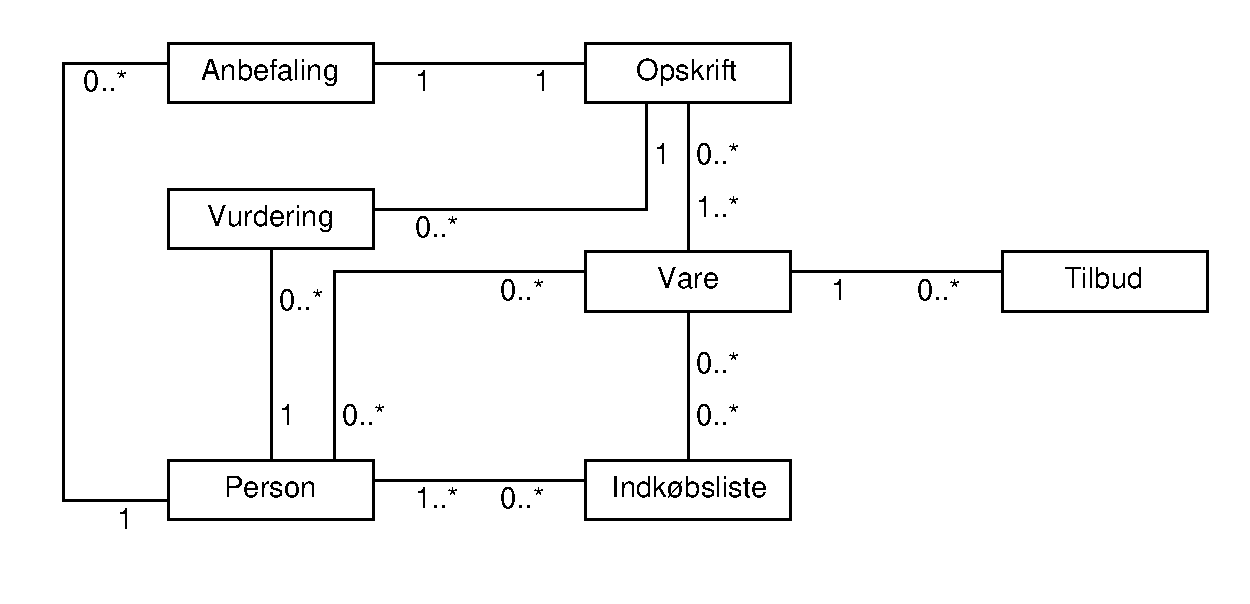
\includegraphics[scale=0.6]{images/Diagrams/klassediagram_model_simple.pdf}
	\caption{Klassediagram over problemområdet.}\label{figur:PDklasse}
\end{figure}

Klassediagrammet som ses på \myref{figur:PDklasse}, beskriver forholdet mellem de forskellige klasser som findes i problemområdet.
Diagrammets sammenhænge er dannet ud fra hændelsestabellen, og beskrivelserne af klasserne.\fxnote{Sørg for at denne model stemmer over ens med modellen vi ender ud med i programmet. I programmet kan vi så henvise til at denne model over klasserne blev brugt til at danne associationerne, imellem klasserne. Der er nemlig ingen henvendelse lige pt, og det kan helt klart bruges. Beskrivelsen nedenfor er næsten identisk med den man finder i Arkitektur - Søren}

Personer kan lave indkøbslister, disse indkøbslister kan være ejet og administreret af enten en eller flere personer.
En indkøbsliste kan bestå af nul til mange varer.
En vare kan være på tilbud i mere end en butik, og derfor have nul til mange tilbud.
En vare kan desuden indgå i en opskrift, og er derfor forbundet med nul til mange.
Desuden har opskrifterne en til mange varer på listen over ingredienser.
Varen kan også være tilføjet til overvågningslisten hos en person, så derfor har personer og varer en nul til mange relation på hinanden.
En person i problemområdet kan give hver opskrift en vurdering, derfor kan personen give nul til mange vurderinger.
En vurdering gives til en opskrift alene, imens en opskrift kan have mange vurderinger, eller ingen vurderinger.
Anbefalinger består af en opskrift, imens personen kan modtage nul til mange anbefalinger.

Ovenstående analyse vil hjælpe til at designe systemets implementering, først foretages dog en analyse af anvendelsesområdet, for at undersøge hvad der er muligt at foretage sig i systemet.

\section{Anvendelsesområde}
Anvendelsesområdet defineres som:

\textit{``En organisation, der administrerer, overvåger eller styrer et problemområde.''}

\subsection{Anvendelseområde analyse}
eTilbudsavis er en organisation der overvåger tilbudsaviser der er tilgængelige online, og giver da mulighed for at foretage søgninger og fremfinde præcise tilbud ud fra en større samling af aviser.
Denne information skal vi bruge til at kunne informere brugerne om relevante tilbud.
Derfor har vi taget kontakt til eTilbudsavisen, og håber på at få lov til at bruge deres API.
Brugerne er personer der overvåger varer, opretter indkøbslister og ser på tilbud samt bedømmer opskrifter.
Brugerne administrerer også hvilke krav og præferencer de har til deres indkøbsliste og derfor også deres opskrifter.
De reagere på og overvåger derfor også anbefalinger som andre brugere har vurderet.
En server skal overvåge og administrere anbefalinger, kunder og databaser.
Serveren skal sørge  for at kunderne har adgang til deres data fra forskellige enheder.
Serveren vil give anbefalinger ved at sammenligne de vurderinger en opskrift har modtaget fra flere brugere.

Klienter er de enheder kunder benytter til at tilgå servicen, dette kan være smartphones, tablets eller computere.

\fxnote{Det hele skal vist bare skrives om :) }

\section{Kravspecifikation}\label{sec:krav}

På baggrund af analysen af problemområdet, anvendelsesområdet og interviewene beskrevet i  \myref{section:interview2} kan der nu opstilles krav til systemet, samt hvad det skal kunne.
Følgende user stories er baseret på brugsmønstrene og funktionerne fra \myref{sec:anvendelses}, samt svarene fra de interviewede.
Som nævnt i \myref{chapter:Metode} benytter vi user stories til at formulere kravspefikationen, da vi benytter Scrum.
\begin{enumerate}
	\item Som en bruger vil jeg kunne oprette indkøbslister.
	\item Som en bruger vil jeg kunne tilføje varer til min(e) indkøbsliste(r).
	\item Som en bruger vil jeg kunne se tilbud.
	\item Som en bruger vil jeg kunne se tilbudsvarer jeg har valgt, deres pris, butik og dato på indkøbslisten.
	\item Som en bruger vil jeg kunne aftjekke en vare fra indkøbslisten.
	\item Som en bruger vil jeg kunne overvåge specifikke vare, og få en notifikation når disse varer kommer på tilbud.
	\item Som en bruger vil jeg kunne finde opskrifter.
	\item Som en bruger vil jeg gerne logge ind.
	\item Som en bruger vil jeg kunne finde opskrifter ud fra anbefalinger til mig.
	\item Som en bruger vil jeg kunne vurdere opskrifter jeg har prøvet.
	\item Som en bruger vil jeg kunne indstille mine præferencer.
	\item Som en bruger vil jeg kunne ekskludere tilbud fra butikskæder som ikke er relevante for mig.
	\item Som en bruger vil jeg kunne dele min indkøbsliste med andre.
	\item Som en bruger vil jeg kunne søge på varer, og finde deres tilbud.
	\item Som en bruger vil jeg kunne tilføje ingredienser for en opskrift til min indkøbsliste.
	\item Som en bruger vil jeg kunne tilgå min indkøbsliste fra min smartphone.
	\item Som en bruger vil jeg kunne skalere opskrifterne til et valgt antal personer.
\end{enumerate}

Disse user stories vil blive designet og implementeret i systemet.
Desuden stilles der yderligere krav til projektet og systemet, bl.a. fra funktionaliteter fundet i \myref{subsec:funktioner}, og fra studieordningen.

\subsection{Krav til systemet}
\begin{enumerate}
\item Der skal benyttes C\# til programmering af systemet.
\item Systemet skal kunne tilgås via forskellige enheder, og gemme information fra enhed til enhed.
\item Systemet skal benytte aktuelle tilbud fra diverse dagligvarebutikker.
\item Systemet skal kunne modtage feedback på de opskrifter brugerne prøver.
\item Systemet skal kunne anbefale opskrifter på baggrund af:
\begin{enumerate}
	\item Madvaner (varieret kost).\fxnote{Dette krav er ikke overholdt, og har aldrig været med i vores overvejelser til udviklingsprocess}
	\item Bedømmelse på opskrift.
\end{enumerate}
\item Systemet skal kunne fjerne forslag om eksempelvis kød til vegetarer ud fra præferencer.
\end{enumerate}

\subsection{Krav til UI (brugergrænseflade)}
\begin{enumerate}
	\item Systemets UI skal være på dansk.
	\item Systemet skal kunne anvendes på forskellige enheder
	\item Systemets UI skal være responsivt og tilpasse sig den anvendte platform.
	\item Brugerne skal synes det er nemt at skabe sig overblik over systemet og navigering heri.
\end{enumerate}

Alle kravene i dette afsnit vil blive taget i betragtning, under design og implementering af systemet.
Slutteligt i rapporten konkluderes der på hvor vidt disse krav er opfyldt, og desuden vil der udføres endnu en række interviews med brugere for at teste deres tilfredsstillelse med systemet.
I de følgende afsnit vil udviklingsprocessen yderligere beskrives, samt designet og implementationerne af løsninger til kravene stillet i dette afsnit.

